\documentclass[12pt]{beamer}
\usetheme{Pittsburgh}
\usecolortheme{crane}
\usepackage{hyperref}
\usepackage[utf8]{inputenc}
\usepackage[spanish,mexico]{babel}

\usepackage{graphicx}
\usebackgroundtemplate%
{%
    
\includegraphics[width=\paperwidth]{Images/pagina_02.jpg}%
}

\title{Mitos y realidades de la seguridad en Java}
\author{Víctor Orozco}
\institute{Nabenik}
\date{\today}

\begin{document}

{
\usebackgroundtemplate{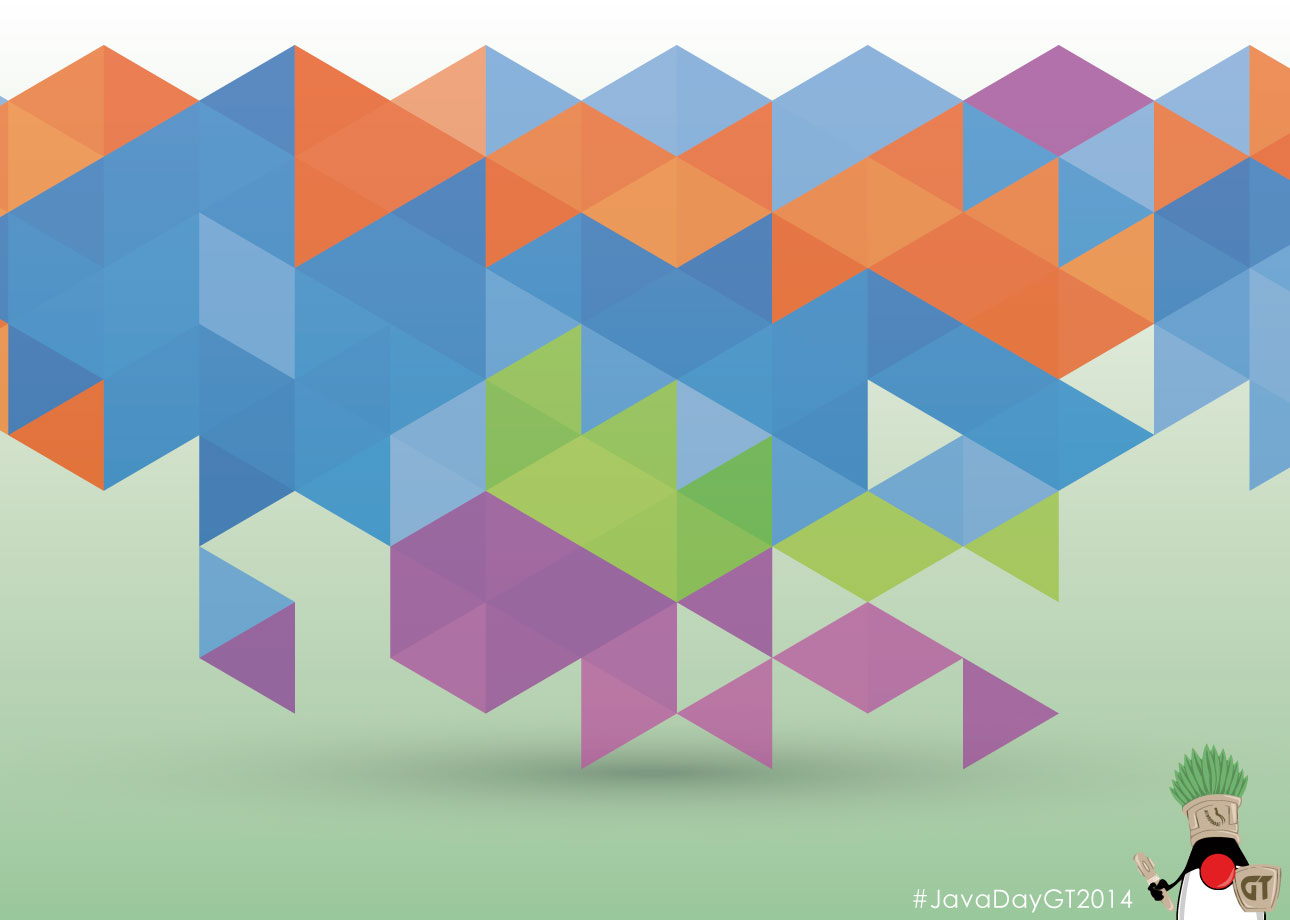
\includegraphics[width=\paperwidth]{Images/portada.jpg}}%
\frame{\titlepage}
}

\section{Estado de Java}

\begin{frame}
\LARGE \centering Disertativa sin código
\end{frame}

\begin{frame}
\begin{figure}
\centering
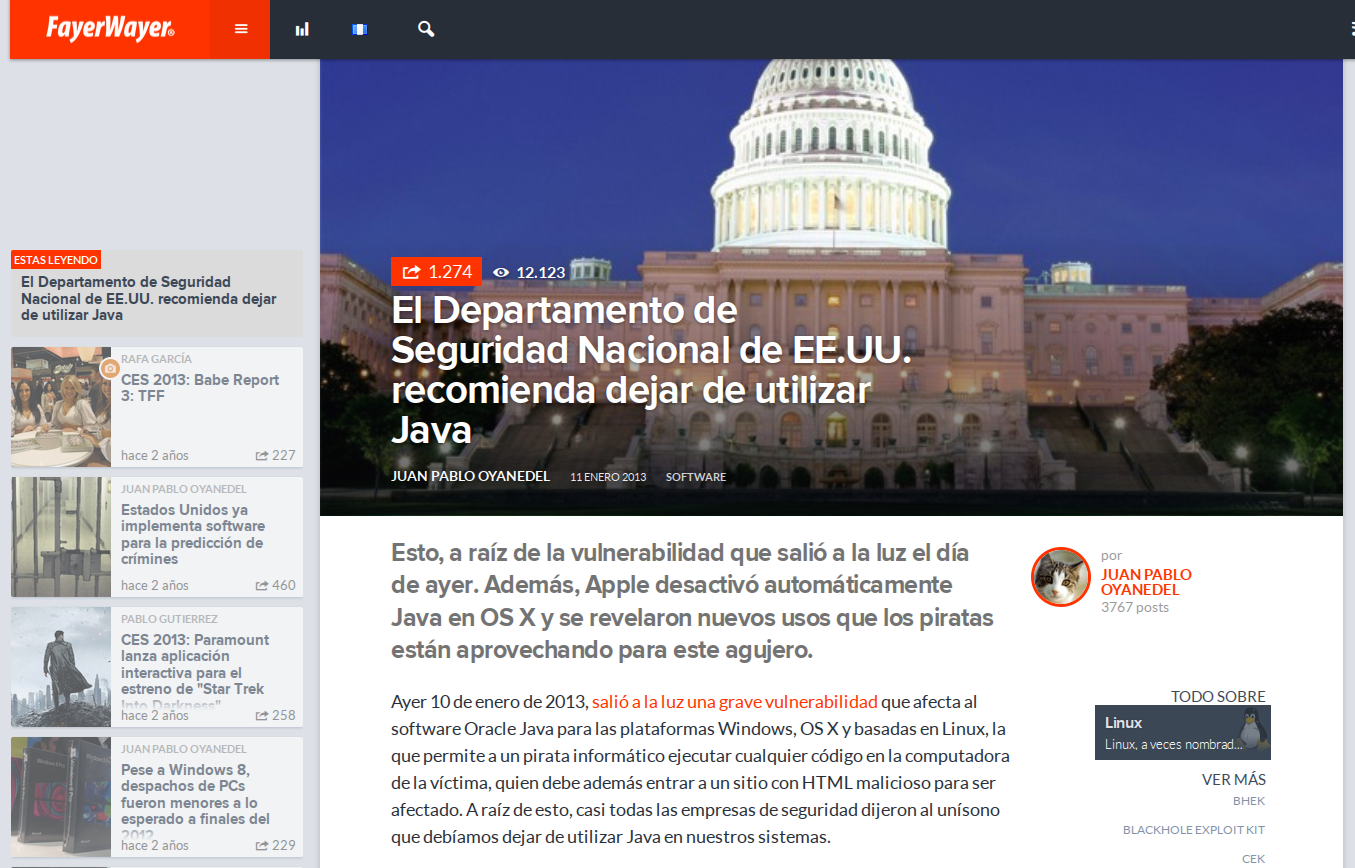
\includegraphics[width=\linewidth]{Images/not1}
\end{figure}
\end{frame}

\begin{frame}
\begin{figure}
\centering
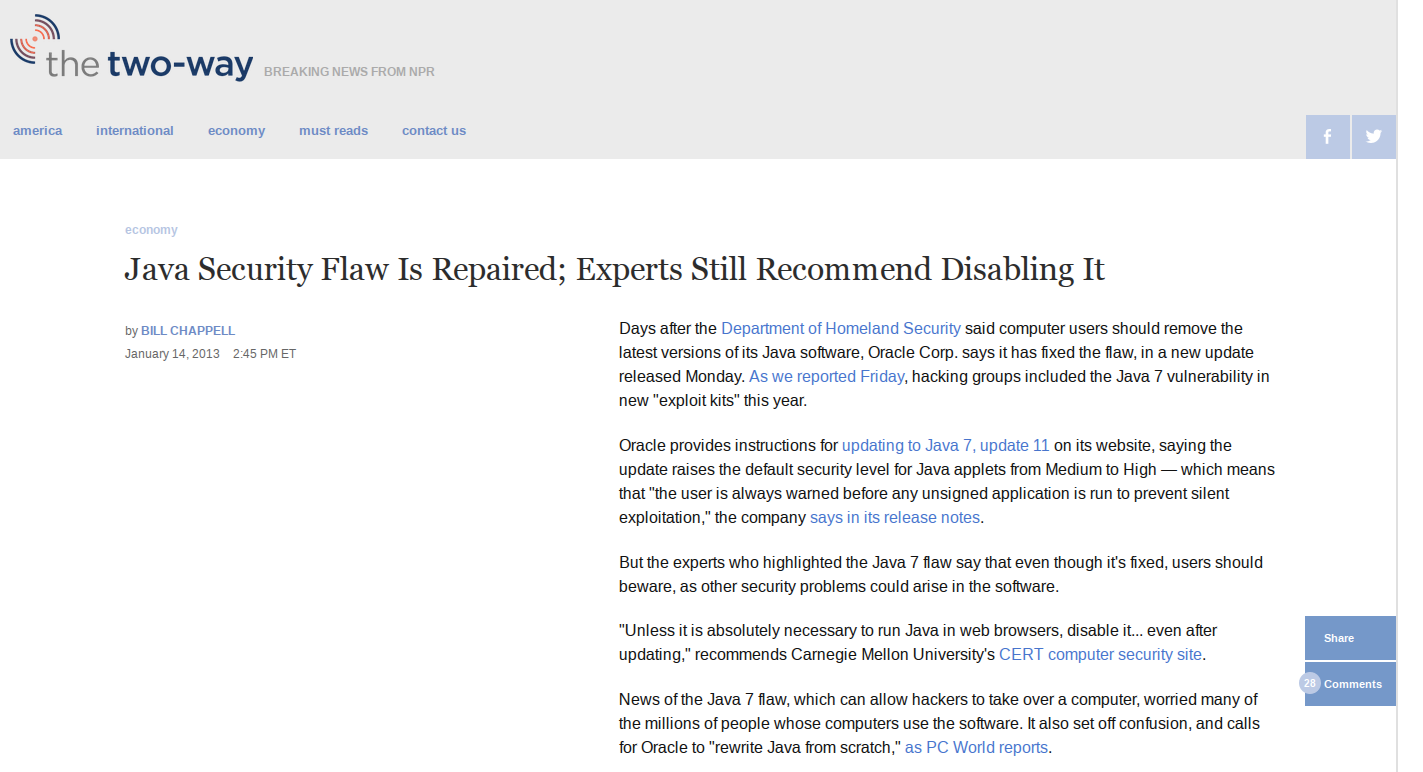
\includegraphics[width=\linewidth]{Images/not2}
\end{figure}
\end{frame}

\begin{frame}
\begin{figure}
\centering
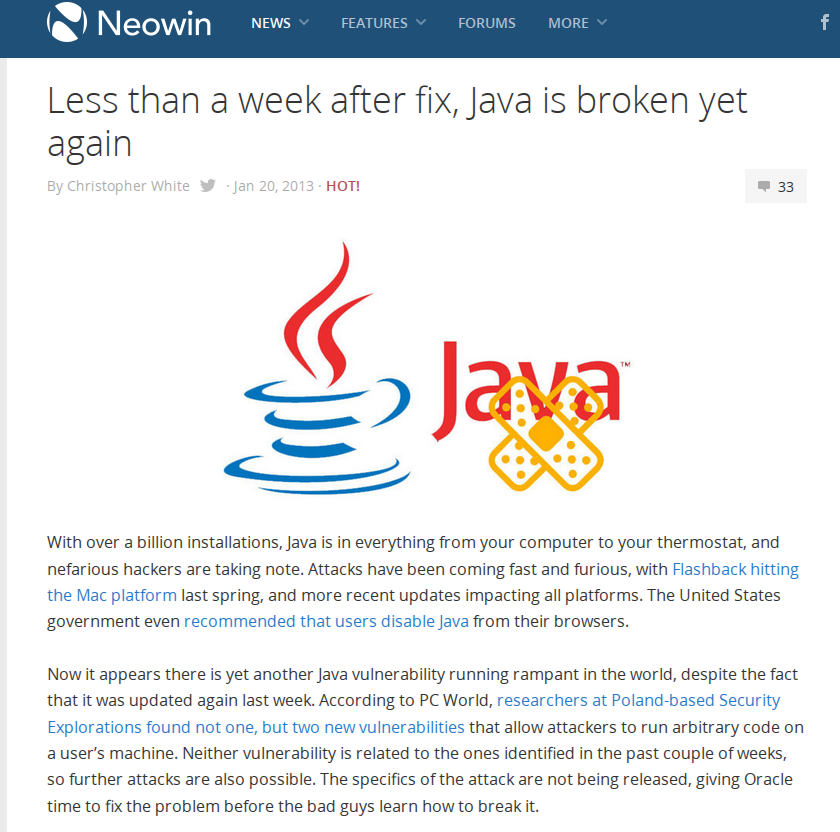
\includegraphics[width=\linewidth]{Images/not3}
\end{figure}
\end{frame}

\begin{frame}
\begin{figure}
\centering
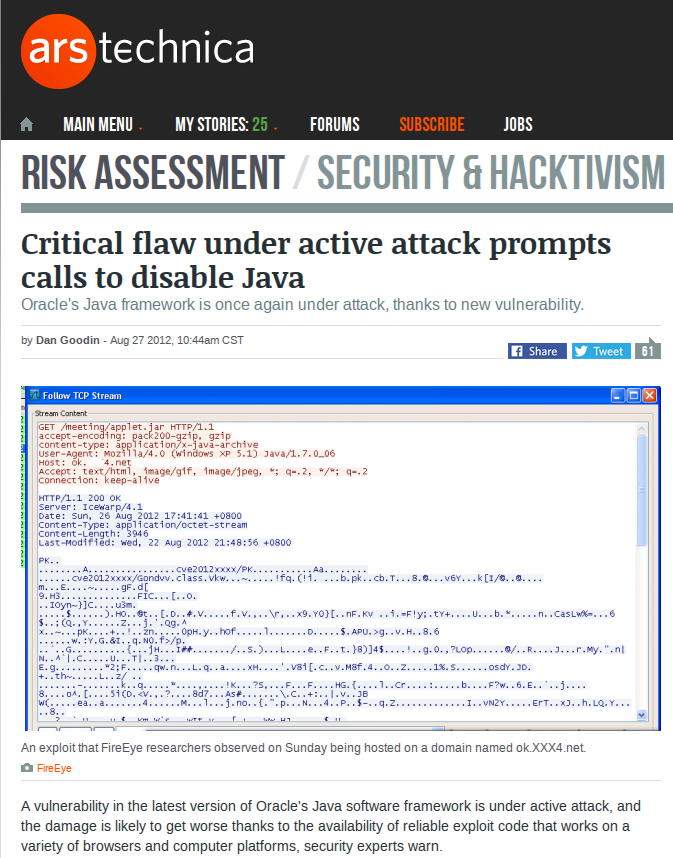
\includegraphics[width=\linewidth]{Images/not4}
\end{figure}
\end{frame}

\begin{frame}
\LARGE \centering ¿Porqué fue importante?
\end{frame}

\begin{frame}
\begin{figure}
\centering
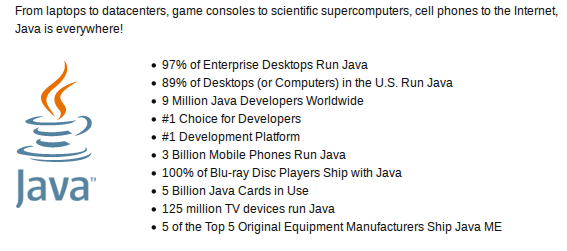
\includegraphics[width=\linewidth]{Images/javapop}
\end{figure}
\end{frame}

\begin{frame}
\begin{figure}
\centering
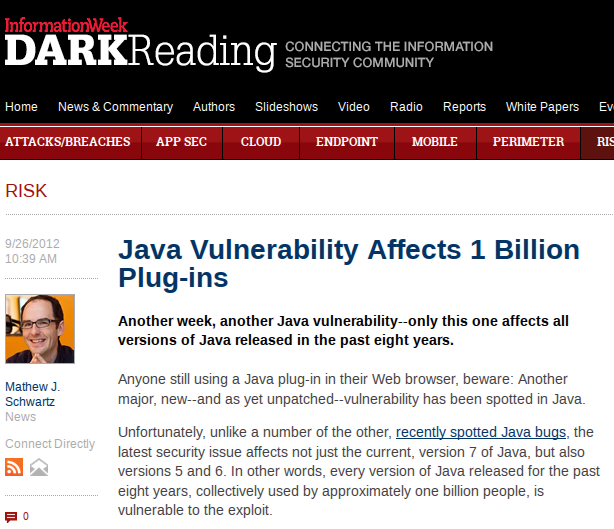
\includegraphics[width=\linewidth]{Images/attacksurface}
\end{figure}
\end{frame}


\begin{frame}
\LARGE \centering Aumento de la superficie de ataque. \\ Write (a exploit) once, run (it) everywhere.
\end{frame}

\begin{frame}{Javas}
\begin{itemize}
\item Java Card
\item Java ME (BD-J, dumbphones)
\item \alert<+>{Java SE (Escritorio, Applets)}
\item Java EE (Web, SOA, personas con corbata)
\end{itemize}
\end{frame}

\begin{frame}
\LARGE \centering ¿Y que pasó desde entonces?
\end{frame}

\begin{frame}{Acciones}
\begin{itemize}
\item Nuevo modelo de lanzamientos
	\begin{itemize}
	\item Limited updates (actualizaciones) - múltiplos de 20
	\item Critical patch updates - Impares en multiplos de 5
	\item \textbf{8u20} 8u25 8u31 8u35 \textbf{8u40} 8u45 \textbf{8u50}
	\end{itemize}
\item Nuevo jefe de seguridad - http://www.securitycurmudgeon.com/2014/04/spotlight-on-java-se-8-security.html
\item Grupo de seguridad en OpenJDK - http://openjdk.java.net/groups/security/
\item Nuevo security track a partir de JavaOne 2013
\end{itemize}
\end{frame}

\begin{frame}
\centering \url{http://java-0day.com/} 11-10-2014
\begin{figure}
\centering
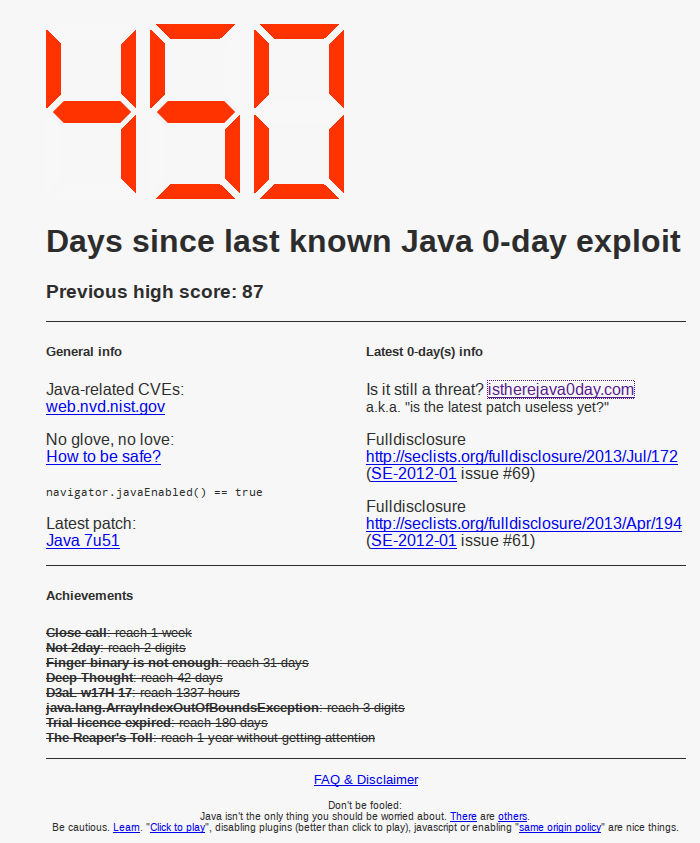
\includegraphics[width=\linewidth]{Images/not5}
\end{figure}
\end{frame}


\section{Buenas practicas}

\begin{frame}
\LARGE \centering ¿Como debo protegerme?
\end{frame}

\begin{frame}
\begin{figure}
\centering
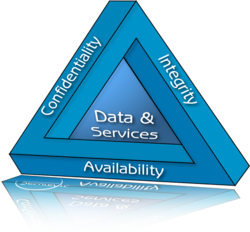
\includegraphics[width=0.5\linewidth]{Images/ciatriad}
\end{figure}
\end{frame}


\begin{frame}
\LARGE \centering -1. Evitar pentesting king/kids
\end{frame}

\begin{frame}
\begin{figure}
\centering
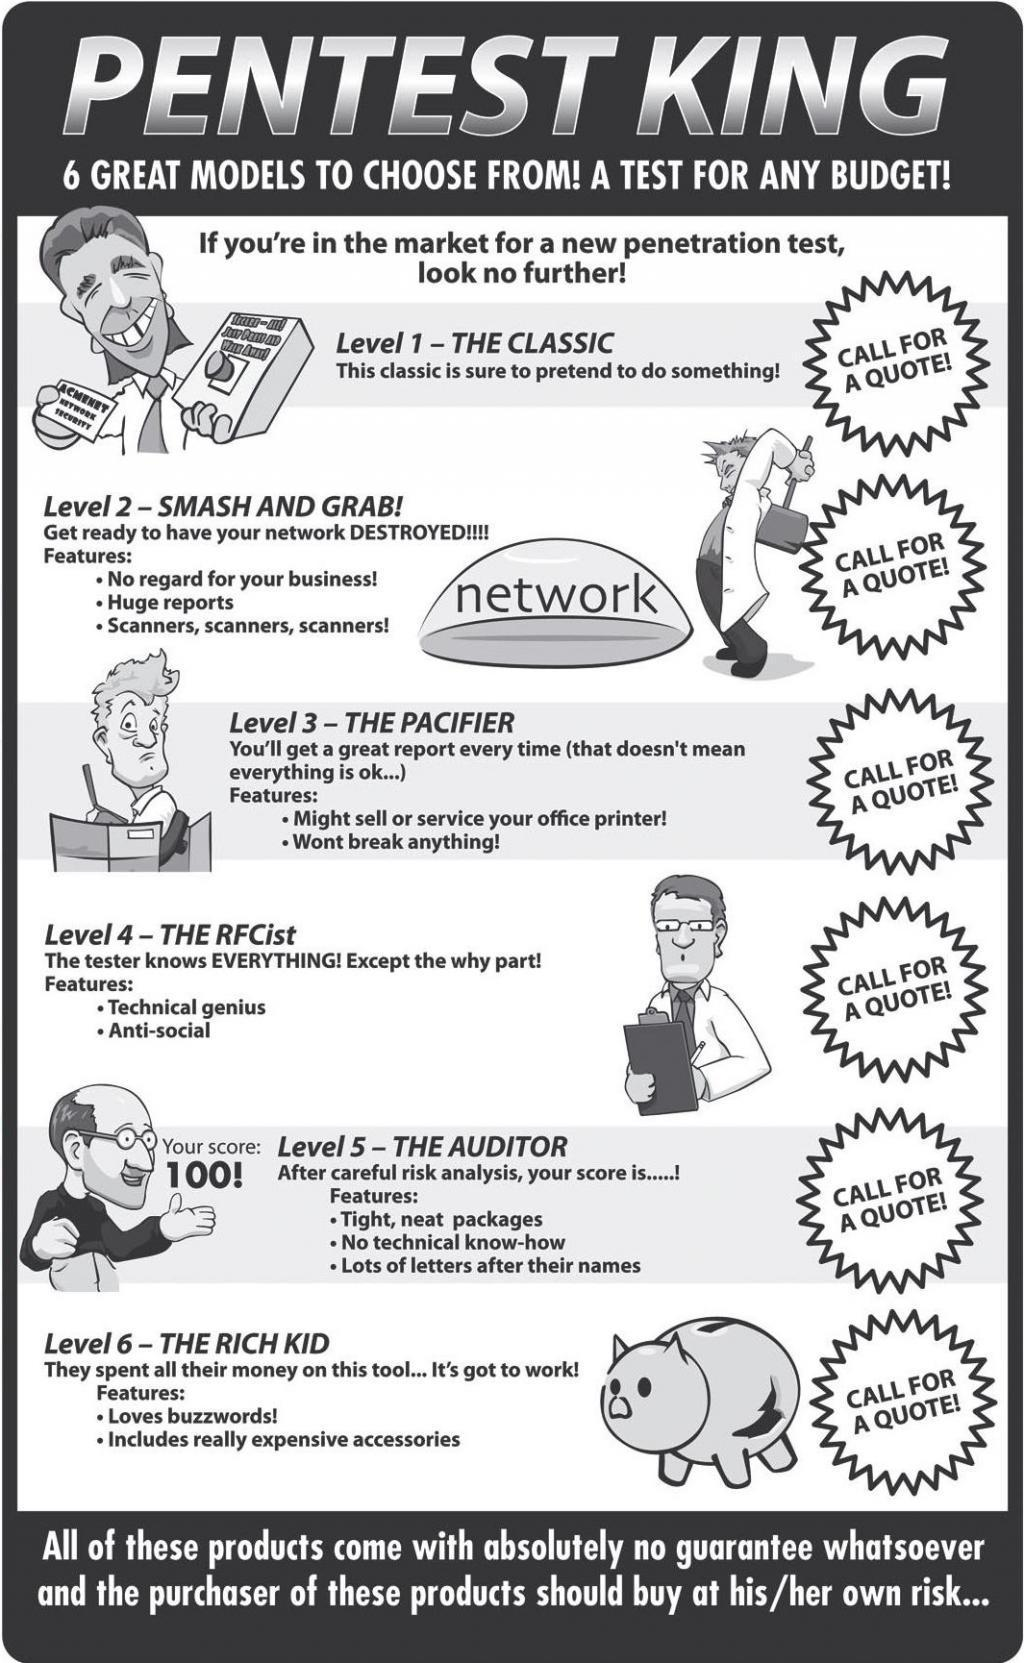
\includegraphics[width=0.6\linewidth]{Images/pentestingkings}
\end{figure}
\end{frame}

\begin{frame}
\LARGE \centering 0. Conociendo NUESTRO java
\end{frame}


\begin{frame}{Javas}
\begin{itemize}
\item \textbf{HotSpot} (Oracle)
\item JRockit (Oracle)
\item OpenJDK (Oracle)
\item Jikes (Eclipse)
\item HP-UX Java (HP)
\item J9 (IBM)
\item Zing (Azul Systems)
\item Zulu (Azul Systems+OpenJDK)
\end{itemize}
\begin{figure}
\centering
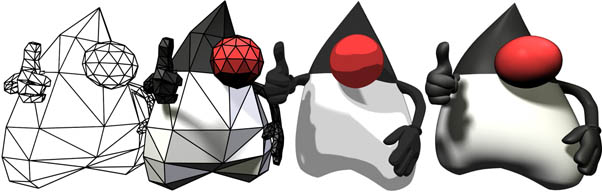
\includegraphics[width=0.6\linewidth]{Images/dukes.jpg}
\end{figure}
\end{frame}

\begin{frame}
\LARGE \centering 1. (Intentar)Ir a la velocidad de los atacantes
\end{frame}

\begin{frame}{Recursos}
\begin{itemize}
\item CVE - \url{http://web.nvd.nist.gov/view/vuln/search-results?query=java\&search\_type=all\&cves=on}
\item Oracle Software Security Assurance - \url{https://blogs.oracle.com/security/}
\item Debian Advisories - \url{https://www.debian.org/security/}
\item RedHat Advisories - \url{https://access.redhat.com/security/updates/advisory}
\end{itemize}
\end{frame}

\begin{frame}
\LARGE \centering 2. Conociendo los modelos de seguridad de Java
\end{frame}

\begin{frame}
\LARGE \centering Autenticación, autorización, sandboxing y firmado de código.
\end{frame}

\begin{frame}{Modelo JavaSE}
\begin{figure}
\centering
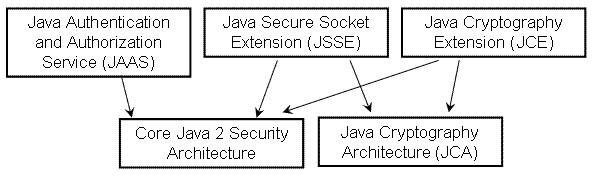
\includegraphics[width=\linewidth]{Images/jsesecurity}
\end{figure}
\end{frame}


\begin{frame}{Modelo JavaEE}
\begin{itemize}
\item Declarativa
	\begin{itemize}
	\item Basado en el contenedor
	\item Modelo de autenticación - Credenciales, OpenID
	\item Modelo de autorización - Basado en roles
	\end{itemize}
\item Programática
	\begin{itemize}
	\item EJBContext
	\item HttpServletRequest
	\end{itemize}
\end{itemize}
\end{frame}

\begin{frame}
\LARGE \centering 3. Programando de forma segura
\end{frame}

\begin{frame}{Buenas practicas de programación}
\begin{itemize}
\item Seguridad = Requerimiento funcional
\item Identificación y corrección de riesgos
\item Patrones de seguridad (reducción de superficie de ataque, privilegios mínimos, defensa en profundidad)
\item Documentación de auditorias
\end{itemize}
\end{frame}


\begin{frame}
\LARGE \centering 4. Desplegando de forma segura
\end{frame}

\begin{frame}{Despliegues seguros}
\begin{itemize}
\item Maven central - \url{http://www.infoq.com/news/2014/08/Maven-SSL-Default}
\item Server JRE - \url{http://www.oracle.com/technetwork/java/javase/7u21-relnotes-1932873.html\#serverjre}
\end{itemize}
\end{frame}




\begin{frame}
\LARGE \centering 5. Utilizando soluciones ya probadas
\end{frame}

\begin{frame}{OWASP Java Enterprise Security API}
  \begin{columns}
      \begin{column}{.5\linewidth}
  	    \begin{figure}
  	    \centering
  	    
\includegraphics[width=0.6\linewidth]{Images/owasp}
  	    \end{figure}
      \end{column}
    \begin{column}{.5\linewidth}
	    \textbf{Tipo:} Biblioteca
	    
	    \textbf{Modo de uso:} Programático
	    
	    \textbf{Características principales:}
	    Criptografía, filtros, reglas de validación, tags JSP, rutinas seguridad
    \end{column}

  \end{columns}
\end{frame}


\begin{frame}{OWASP Java Encoder}
  \begin{columns}
      \begin{column}{.5\linewidth}
  	    \begin{figure}
  	    \centering
  	    
\includegraphics[width=0.6\linewidth]{Images/owasp}
  	    \end{figure}
      \end{column}
    \begin{column}{.5\linewidth}
	    \textbf{Tipo:} Biblioteca
	    
	    \textbf{Modo de uso:} Programático
	    
	    \textbf{Características principales:}
	    XSS
    \end{column}

  \end{columns}
\end{frame}


\begin{frame}{Bouncy Castle}
  \begin{columns}
      \begin{column}{.5\linewidth}
  	    \begin{figure}
  	    \centering
  	    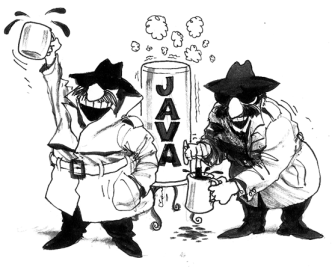
\includegraphics[width=0.6\linewidth]{Images/bouncyjava.png}
  	    \end{figure}
      \end{column}
    \begin{column}{.5\linewidth}
\textbf{Tipo:} Biblioteca

\textbf{Modo de uso:} Programático

\textbf{Características principales:}
API Ligera (funciona con JME)
Proveedor para Java Cryptography Extension
Generador y procesador de certificados (S/MIME, OCSP, TSP, CMP, OPENPGP)
Jar firmado y compatible con Hotspot
    \end{column}

  \end{columns}
\end{frame}

\begin{frame}{Jasypt}
  \begin{columns}
      \begin{column}{.5\linewidth}
  	    \begin{figure}
  	    \centering
  	    
\includegraphics[width=0.6\linewidth]{Images/jasypt.png}
  	    \end{figure}
      \end{column}
    \begin{column}{.5\linewidth}
\textbf{Tipo:} Biblioteca

\textbf{Modo de uso:} Programático

\textbf{Características principales:}
API Ligera (funciona con JME), 
Estándares avanzados de seguridad, 
Integración automática con Hibernate, Spring y Spring Security, 
Cifrado de alto rendimiento, 
A diferencia de bouncy castle, Jasypt se enfoca solo en java
    \end{column}

  \end{columns}
\end{frame}

\begin{frame}{Spring Security}
  \begin{columns}
      \begin{column}{.5\linewidth}
  	    \begin{figure}
  	    \centering
  	    
\includegraphics[width=0.6\linewidth]{Images/spring.png}
  	    \end{figure}
      \end{column}
    \begin{column}{.5\linewidth}
\textbf{Tipo:} Biblioteca

\textbf{Modo de uso:} Programático+Declarativo

\textbf{Características principales:}
Integración automática con spring,
Soporte para inyección de dependencias,
Acoplamiento debil, los componentes son facilmente reemplazables,
Expression language (reglas),
Autorización de peticiones HTTP,
Autenticación externa (LDAP, JDBC, Kerberos, AD),
Encripción de passwords,
Tags
    \end{column}

  \end{columns}
\end{frame}

\begin{frame}{Apache Shiro}
  \begin{columns}
      \begin{column}{.5\linewidth}
  	    \begin{figure}
  	    \centering
  	    
\includegraphics[width=0.6\linewidth]{Images/shiro.jpg}
  	    \end{figure}
      \end{column}
    \begin{column}{.5\linewidth}
\textbf{Tipo:} Framework

\textbf{Modo de uso:} Programático+Declarativo

\textbf{Características principales:}
Autenticación y autorización basada en roles,
Criptografía,
Administración de sesiones,
Autenticación externa (LDAP, JDBC, Kerberos, AD) y soporte para Single Sign On,
Pocas dependencias,
Acoplamiento debil, componentes fácilmente reemplazables.
    \end{column}

  \end{columns}
\end{frame}

\section{Fin}

\begin{frame}{Gracias}
\begin{itemize}
\item E-mail: tuxtor@shekalug.org
\item Blog: http://tuxtor.shekalug.org
\item Twitter: @tuxtor
\item Fuentes: http://github.com/tuxtor/slides
\end{itemize}
\begin{center}

\includegraphics[width=0.1\linewidth]{Images/cclogo}
\\
This work is licensed under a Creative Commons Attribution-ShareAlike 3.0 Guatemala License.
\end{center}
\end{frame}
\end{document}
